\section{Motivation and Background}
\label{sec:motivation_background}

\noindent The Web is emerging as a medium for connecting distributed applications, becoming---more than an information system---into a platform that
supports the operation of a huge ecosystem of services \cite{Webber:2010a}, which are built under different architectures and design philosophies. Leonard Richardson has proposed in \cite{Richardson:2008} a schema for classifying services on the Web, defining three maturity levels (plus a zero level). Each of the levels represents one element of what Richardson calls \emph{the technology stack for web services}: URI, HTTP, Hypermedia (see Figure \ref{richardsonModel}). This way, services are classified according to the technologies that supports their operation.

\begin{figure}[H]
\center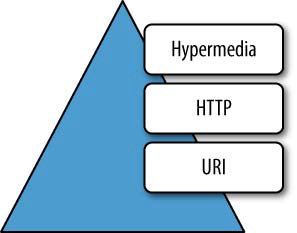
\includegraphics[scale=0.6]{images/WS-MaturityModel}

\caption{Richardson's service maturity model. {\scriptsize source: \cite{Webber:2010a}}}
\label{richardsonModel}
\end{figure}

\begin{itemize}
\item \emph{Level zero services}: services at this level are characterized by having an unique URI and using only one HTTP method (typically \texttt{POST}). At this level we find the XML-RPC services \cite{Laurent:2001} and most of the SOAP services. 
\item \emph{Level one services (URI support)}: At this level, services employ various URIs but only one HTTP method. In contrast to level zero services---which tunnel all the interactions through a unique and rather complex resource---services at level one expose multiple logical resources. However services at this level tunnel their actions by inserting parameters and values into a URI, which is then transmitted to a remote service (via \texttt{HTTP GET} typically). According to Richardson, most of the services out there that claim to be RESTful are actually level one services.
\item \emph{Level two services (HTTP support)}: this level deals with services that host many resources, each of which is addressable through its own URI. Additionally level two services support various HTTP methods on their resources. This level includes CRUD-like (\emph{Create}, \emph{Read}, \emph{Update}, \emph{Delete}) services, such as the Amazon cloud storage system (\emph{Amazon S3}: \href{http://aws.amazon.com/es/s3/} {http://aws.amazon.com/es/s3/}).
\item \emph{Level three services (Hypermedia support)}: At this level, we find real RESTful services: those having the features of level two services, plus supporting the notion of \emph{hypermedia as the engine of application state} (HATEOAS), that is to say, the representations of the resources hosted by the service contain controls that enable consumers to access related resources. This way the service leads its users through a trail of resources, causing application state changes in consequence. Examples of this kind of services include the Web and the REST API of \emph{Netflix} (\href{http://developer.netflix.com/docs/REST_API_Conventions} {http://developer.netflix.com/docs/REST\_{}API\_{}Conventions}). 
\end{itemize}

A research conducted by Maleshkova et al. \cite{Maleshkova:2010} reports that, despite the apparent spreading of RESTful services in the Web, there are actually few services that supports all the tenets and constraints of REST. The authors of this study have analyzed by hand 222 web APIs, randomly chosen from the \emph{Programmable Web }API directory\emph{} \footnote{Available at:\emph{ }\href{http://www.programmableweb.com/}{http://www.programmableweb.com/}}. The results that arose from their analysis, evidence that only 32\% of services could be considered---at least approximately---REST services (i.e., services from levels two and three in the Richardson maturity model), while the remaining 68\% was RPC and hybrid services (i.e., services from levels zero and one, according to the same model).

The study of Maleshkova also states that service development is driven by the particular criteria of its creators, rather than well-established standards and rules. Similarly, service documentation (specially REST service documentation) is not supported on interface description languages such as WSDL (for SOAP services), but it is provided as HTML pages, which have no regular or standard structure. Therefore, the use of web services requires a cumbersome manual process which additionally hinders the execution of discovery, composition and invocation procedures. In this regard, some initiatives have been fostered, seeking the definition of standard formats for describing REST services. That is the case of WADL (\emph{Web Application Description Language}) \cite{W3C:2009}, a language intended for specifying HTTP-based web services and applications.

A WADL descriptor (or contract) is a document that specifies the set resources hosted by a service, as well as their associated URI templates, the HTTP methods the service supports and the representations it is able to receive and deliver. Just like WSDL for SOAP services, WADL enables automatic building of services clients, making them easier to consume and accessible to developers. Nonetheless, WADL descriptors merely describe the static view of services and applications, neglecting the user-resources interaction dynamics, which is better specified by hypermedia and media types. Consequently, as stated in \cite{Webber:2010b}, this kind of descriptor is suitable only for CRUD-like REST services (Level two services) whose functionality is limited to manipulate records from a data set.

So far, WADL has been poorly adopted as description language for REST services. Instead other studies have been conducted for defining service descriptors that include semantic metadata, which aim to enable the automatic discovery and composition of services. Semantic annotations make it possible for intelligent agents to understand the services functionality, and establishing service relationships at the semantic level (e.g., similarity, partial matching, and membership\cite{Paolucci:2002}).

In this regard the academic community has came up with proposals like hRESTS \cite{Kopecky:2008}---an HTML-based description microformat that allows specifying the services functional attributes, like its operations, inputs and outputs---, along with its extensions SA-REST \cite{Sheth:2007} and MicroWSMO \cite{Kopecky:2009}, which enable the semantic annotation of hREST descriptors.

Another approach to REST API description is \emph{RESTdesc}, proposed by Verborgh et al. in \cite{Verborgh:2013}. RESTdesc provides a functionality-centered format for semantic description of REST services, as well as an automatic discovery mechanism based on inference with logic rules specifying the capabilities of these resources. According to the authors of RESTdesc, the approach they propose is supported on well known technologies such as HTTP and RDF/Notation3 and is grounded on the hypermedia and \emph{Linked Data} concepts, from which defines and leverages relationships between different services specifications, enabling intelligent agents to automatically discover and compose services.

Since, in general terms, there is a sort of barrier regarding the adoption of new formats for specifying the web service semantics, our proposal intends to use the information currently available in service description documents---i.e., WSDL interfaces for SOAP services and HTML documents for XML-RPC and REST services---in order to abstract a knowledge representation based on the content of such documentation, from which it would be possible to establish semantic similarity relations between services. This proposal is founded on three main processes: 

\begin{enumerate}
\item Extraction of technical information related to service functionality. 
\item Analysis of the extracted information for identifying conceptual categories
the services they comprise. 
\item Deriving a taxonomy from the categories obtained in process (2). 
\end{enumerate}

% Nowadays the amount of information and resources available on the Web is huge and ever increasing, so that it has exceeded our ability for locating and accessing the resources we need. This way, increasingly sophisticated computational tools are required for organizing, searching and understanding those resources, beyond the traditional information indexing and retrieval approaches.
% 
% Semantic annotation, is one of the core concepts of the current proposal. It aims to make explicit for machines, the meaning (the semantics) of content and resources available in large repositories of information. This latter constitutes one of the requirements to meet to finally materializing the Semantic Web. The semantic annotation procedure is commonly supported in formal representation of knowledge, as the aforementioned ontologies, and for services, consists in associating ontological entities to the terms defining the attributes of the service in its descriptor document [8], allowing for instance, for service search engines to effectively comprehend (on a semantic level) both the services functionality as the service’s  clients requests, enabling them to accurately respond to service inquiries.
% 
% Traditionally, this semantic annotation procedure must be performed by hand by service designers and developers or in a collaborative way by service users (conceiving a sort of folksonomy of services). In both cases, the large and growing amount of services, along with the lack of knowledge regarding semantic description methods for services and the scarceness of suitable domain ontologies, has overwhelmed the human ability for performing this semantic annotation task. Additionally, the human intervention in marking up the services descriptors with ontological entities involves a very expensive process in terms of time, effort and resources. In this regard, the focus of the present approach is on leveraging current techniques taken from the fields of machine learning, information retrieval and knowledge discovery, for automating the semantic annotation of web services. The next section will deal the revision of some previous works regarding the problem being tackled herein.